\documentclass[tikz,border=8pt]{standalone}
% Shared look for every TikZ diagram. Load with \input{../../tools/tikz-style.tex}
\usepackage[T1]{fontenc}
\usepackage{lmodern}
\renewcommand{\sfdefault}{lmr}  % diagrams use the same serif as the text
\usetikzlibrary{arrows.meta, positioning, shapes.geometric, calc, fit, backgrounds}
\definecolor{cblue}{HTML}{4C78A8}
\definecolor{corange}{HTML}{F58518}
\definecolor{cgreen}{HTML}{54A24B}
\definecolor{cred}{HTML}{E45756}
\definecolor{cpurple}{HTML}{B279A2}
\definecolor{cgrey}{HTML}{6B6B6B}
\tikzset{
  every picture/.style={font=\sffamily, line width=1.2pt},
  box/.style={draw=#1, fill=#1!12, rounded corners=4pt, align=center, inner sep=7pt, minimum height=1.1cm},
  box/.default=cgrey,
  arrow/.style={-{Stealth[length=3mm]}, draw=cgrey, line width=1.4pt},
  title/.style={font=\sffamily\bfseries\Large},
  note/.style={font=\sffamily\small, text=cgrey, align=center},
}
\AtBeginDocument{\hyphenpenalty=10000 \exhyphenpenalty=10000}

% The two numbers that describe the robot's motion: forward speed v along the heading (straight arrow) and turn rate
% omega, how fast the heading turns (curved arrow, positive = left).
\begin{document}
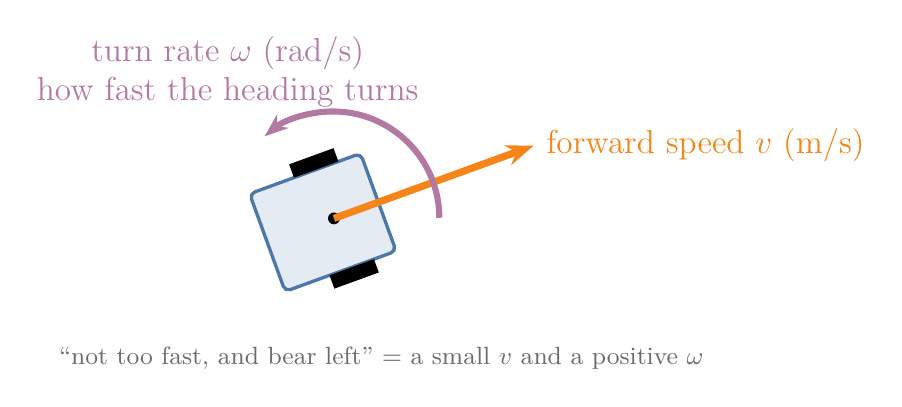
\begin{tikzpicture}[scale=3, every node/.append style={font=\large}]
  \begin{scope}[rotate=20]
    \draw[cblue, fill=cblue!15, rounded corners=2pt] (-0.3,-0.22) rectangle (0.2,0.22);
    \fill[black] (-0.1,0.22) rectangle (0.1,0.28); \fill[black] (-0.1,-0.28) rectangle (0.1,-0.22);
    \fill[black] (0,0) circle (0.025);
    \draw[-{Stealth[length=3.5mm]}, corange, line width=2.6pt] (0,0) -- (0.9,0) node[right] {forward speed $v$ (m/s)};
    \draw[-{Stealth[length=3mm]}, cpurple, line width=2.2pt] (0.42,-0.15) arc (-20:110:0.45);
  \end{scope}
  \node[cpurple, align=center] at (-0.45,0.62) {turn rate $\omega$ (rad/s)\\how fast the heading turns};
  \node[note, anchor=north] at (0.2,-0.5) {``not too fast, and bear left'' $=$ a small $v$ and a positive $\omega$};
\end{tikzpicture}
\end{document}
